\section{Дифференциальное исчисление функций одной переменной}
    \subsection{Производная функции}
        В следующих определениях предполагается, что $f(x)$ определена в $B(x_0)$.
        \begin{definition}
            Производной функции $f(x)$ в точке $x_0$ называется (если он существует) предел
             \[f^{\prime}(x_0):=\lim\limits_{\Delta x\to 0}\frac{f(x_0+\Delta x)-f(x_0)}{\Delta x}\]
        \end{definition} 
        \begin{definition}
            Производной функции $f(x)$ в точке $x_0$ по множесту $A$ называется (если он существует) предел 
            \[f_A^{\prime}(x_0):=\lim\limits_{A \ni \Delta x\to 0}\frac{f(x_0+\Delta x)-f(x_0)}{\Delta x}\]
            Если $A=(x_0-\Delta x, x_0)$ или $(x_0,x_0+\Delta x)$, то пишут $f_{-}^{\prime}(x_0)$ или $f_{+}^{\prime}(x_0)$. 
        \end{definition} 
        \begin{comm} Если обозначить $\Delta x=x-x_0$, то
            \[\lim\limits_{\Delta x\to 0}\frac{f(x_0+\Delta x)-f(x_0)}{\Delta x}=\lim\limits_{x\to x_0}\frac{f(x)-f(x_0)}{x-x_0}\]
        \end{comm} 
        \begin{theorem}
            Если существует производная функции $f(x)$ в точке $x_0$, то $f(x)$ непрерывна в точке $x_0$.
        \end{theorem} 
         \begin{proof}
            \[\exists\ f'(x)=\lim\limits_{x\to x_0}\frac{f(x)-f(x_0)}{x-x_0} \Rightarrow \frac{f(x)-f(x_0)}{x-x_0}=f'(x)+\bar{\bar{o}}{(1)}\]
            Так как $x-x_0=\bar{\bar{o}}{(1)}$ при $x\to x_0$, то это равенство можно записать в виде:
            \[f(x)-f(x_0)=(f'(x)+\bar{\bar{o}}{(1)})(x-x_0)=\bar{\bar{o}}{(1)}\]
            Значит
            \[\lim\limits_{x\to x_0}f(x)=f(x_0)\]
        \end{proof}
        %\begin{proof}
        %    временно очев
        %\end{proof}
        \begin{theorem}
            Если у функций $f(x)$ и $g(x)$ существуют производные в точке $x_0$, то $\forall C\in \R$ выполнено:
            \begin{enumerate}
                \item $\exists\ (Cf(x_0))^{\prime}=C f^{\prime}(x_0)$.
                \item $\exists\ (f(x_0)\pm g(x_0))^{\prime}=f^{\prime}(x_0)\pm g^{\prime}(x_0)$.
            \end{enumerate}
        \end{theorem} 
        \begin{theorem}
            Если $\exists\ f^{\prime}(x_0)$ и $\exists\ g^{\prime}(x_0)$, то $\exists\ (f(x_0)g(x_0))^{\prime}=f^{\prime}(x_0)g(x_0)+g^{\prime}(x_0)f(x_0)$.
        \end{theorem} 
        \begin{proof}
            \begin{multline*}
                \lim\limits_{x\to x_0}\frac{f(x)g(x)-f(x_0)g(x_0)}{x-x_0}=\\
                =\lim\limits_{x\to x_0}\frac{f(x)g(x)-f(x_0)g(x)+f(x_0)g(x)-f(x_0)g(x_0)}{x-x_0}=\tab[2cm]\\
                \tab[2cm]=\lim\limits_{x\to x_0}\frac{(f(x)-f(x_0))g(x)}{x-x_0}+\lim\limits_{x\to x_0}\frac{(g(x)-g(x_0))f(x_0)}{x-x_0}=\\
                =f^{\prime}(x_0)g(x_0)+g^{\prime}(x_0)f(x_0)
            \end{multline*}
            в последнем переходе используется непрерывность $g(x)$\\
            ($\exists\ g^{\prime}(x_0) \Rightarrow g(x)$ непрерывна в точке $x_0$).
        \end{proof} 
        \begin{theorem}
            Если $\exists\ f^{\prime}(x_0),\ \exists\ g^{\prime}(x_0)$ и $g(x_0)\ne 0$, то
            \[\exists\ (\frac{f(x_0)}{g(x_0)})^{\prime}=\frac{f^{\prime}(x_0)g(x_0)-f(x_0)g^{\prime}(x_0)}{g^2(x_0)}\]
        \end{theorem} 
        \begin{proof}
            \begin{multline*}
                \lim\limits_{x\to x_0}\frac{\frac{f(x)}{g(x)}-\frac{f(x_0)}{g(x_0)}}{x-x_0}=\lim\limits_{x\to x_0}\frac{f(x)g(x_0)-f(x_0)g(x)}{g(x)g(x_0)(x-x_0)}=\\
                =\lim\limits_{x\to x_0}\frac{f(x)g(x_0)-f(x_0)g(x_0)+f(x_0)g(x_0)-f(x_0)g(x)}{g(x)g(x_0)(x-x_0)}=\tab[1cm]\\
                \tab[2.5cm]=\lim\limits_{x\to x_0}\frac{(f(x)-f(x_0))g(x_0)-(g(x)-g(x_0))f(x_0)}{g(x)g(x_0)(x-x_0)}=\\
                =\frac{f^{\prime}(x_0)g(x_0)-g^{\prime}(x_0)f(x_0)}{g^2(x_0)}
            \end{multline*}
            в последнем переходе используется непрерывность $g(x)$.
        \end{proof} 
        \begin{theorem}
            Пусть $y=f(x),\ y_0=f(x_0),\ \exists\ f^{\prime}(x_0),\ \exists\ g^{\prime}(y_0)$. Тогда
            \[\exists\ (g(f(x_0)))^{\prime}=g^{\prime}(f(x_0))f^{\prime}(x_0)\]
        \end{theorem}
        \begin{proof}
            Пусть $x_n\to x_0,\ f(x_n)\to f(x_0)$ и $f(x_n)\ne f(x_0)$. Тогда 
            \begin{multline*}
                (g(f(x_0)))^{\prime}=\lim\limits_{x_n\to x_0}\frac{g(f(x_n))-g(f(x_0))}{x_n-x_0}=\\
                =\lim\limits_{x_n\to x_0}\frac{g(f(x_n))-g(f(x_0))}{f(x_n)-f(x_0)}\cdot \frac{f(x_n)-f(x_0)}{x_n-x_0}=g^{\prime}(f(x_0))f^{\prime}(x_0)
            \end{multline*}
            Остался случай, когда в любой окрестности $x_0$ есть бесконечно много точек, в которых $f(x_n)=f(x_0)$. Тогда
            \[f^{\prime}(x_0)=\lim\limits_{x_n\to x_0}\frac{f(x_n)-f(x_0)}{x_n-x_0}=0\]
            $\Rightarrow g^{\prime}(f(x_0))f'(x_0)=0$
        \end{proof}  
        %\begin{comm}
        %    \[\lim\limits_{x_n\to x_0}\frac{g(f(x_n))-g(f(x_0))}{x_n-x_0}=0\] 
        %    (Использовалось в доказательстве)
        %\end{comm}
        \begin{example}
            $(f(g(h(a(x)))))^{\prime}=f^{\prime}(g(h(a(x))))\cdot g^{\prime}(h(a(x)))\cdot h^{\prime}(a(x))\cdot a^{\prime}(x)$
        \end{example}
    \subsection{Дифференцируемые функции}
        \begin{definition}
            Разность $\Delta x=x-x_0$ называется приращением аргумента. Разность $f(x_0+\Delta x)-f(x_0)$ называется полным приращением функции.
        \end{definition} 
        \begin{definition}
            Пусть $f(x)$ определена в $B(x_0)$. Если $\exists\ A\in \R$ такое, что
            \[f(x_0+\Delta x)-f(x_0)=A \Delta x+\bar{\bar{o}}{(\Delta x)}\]
            то $f(x)$ называется дифференцируемой в точке $x_0$, а главная линенйная часть приращения функции $A \Delta x$ называется (первым) дифференциалом $f(x)$ в точке $x_0$, его обозначают $df=A\Delta x$.\\
            Если функция $f(x)$ дифференцируема на $X\subset \R$, то пишут $f(x)\in \mathcal{D}(X)$
        \end{definition} 
        \begin{theorem}
            $f(x)\in \mathcal{D}(x_0) \Leftrightarrow \exists\ f^{\prime}(x_0)$.
        \end{theorem}
        \begin{proof}\tab
            \begin{itemize}
                \item[$(\Rightarrow)$]: $f(x_0+\Delta x)-f(x_0)=A\Delta x+\bar{\bar{o}}{(\Delta x)}$, значит
                \[\frac{f(x_0+\Delta x)-f(x_0)}{\Delta x}=A+\bar{\bar{o}}{(1)}\Rightarrow \exists\ f^{\prime}(x_0)=\lim\limits_{\Delta x\to 0}\frac{f(x_0+\Delta x)-f(x_0)}{\Delta x}=A\]
                \item[$(\Leftarrow)$]: $\exists\ f^{\prime}(x_0)$, значит
                \[f^{\prime}(x_0)=\lim\limits_{\Delta x\to 0} \frac{f(x_0+\Delta x)-f(x_0)}{\Delta x} \Rightarrow f(x_0+\Delta x)-f(x_0)=f^{\prime}(x_0)\Delta x+\bar{\bar{o}}{(\Delta x)}\] 
            \end{itemize}            
        \end{proof}  
        \begin{comm}\tab
            \begin{enumerate}
                \item $df=f^{\prime}(x_0)\Delta x$
                \item $dx=x^{\prime}\Delta x=\Delta x \Rightarrow df=f^{\prime}(x)dx$
            \end{enumerate}
        \end{comm}  
        \begin{examples}\tab
            \begin{enumerate}
                \item $y=y(x)\ dy=y^{\prime}(x)\ dx \Leftrightarrow dx=\cfrac{1}{y^{\prime}(x)}\ dy$
                \item $x^2+y^2=1 \Rightarrow y=\sqrt{1-x^2}\\
                2x\ dx+2y\ dy=0 \Leftrightarrow dy=-\cfrac{x}{y}\ dx=-\cfrac{x}{\sqrt{1-x^2}}\ dx$.
                \item $\begin{cases}
                    x=x(t),\\
                    y=y(t).       
                \end{cases}$\
                $\begin{cases}
                    dx=x^{\prime}_t\ dt,\\
                    dy=y^{\prime}_t\ dt.       
                \end{cases}$\
                $dy=\cfrac{y^{\prime}_t}{x^{\prime}_t}\ dx$\tab
                $\begin{cases}
                    y^{\prime}_x=\cfrac{y^{\prime}_t}{x^{\prime}_t},\\
                    x=x(t).       
                \end{cases}$
            \end{enumerate}
        \end{examples}
        \begin{theorem} (Теорема о производной обратной функции)\\
            Пусть $\exists\ y^{\prime}=f^{\prime}(x_0),\ f^{\prime}(x_0)\ne 0$. Тогда $\exists\ x=f^{-1}(y)$ и 
            \[(f^{-1}(y_0))^{\prime}=\frac{1}{f^{\prime}(x_0)}\]
        \end{theorem} 
        \begin{proof}
            \[(f^{-1}(y_0))^{\prime}=\lim\limits_{y\to y_0}\frac{f^{-1}(y)-f^{-1}(y_0)}{y-y_0}=\lim\limits_{x\to x_0}\frac{x-x_0}{f(x)-f(x_0)}=\frac{1}{f^{\prime}(x_0)}\]
        \end{proof} 
    \subsection{Производные элементарных функций}
        \begin{enumerate}
                \item $(e^x)^{\prime}=e^x$
                \[\lim\limits_{\Delta x\to 0}\frac{e^{x_0+\Delta x}-e^{x_0}}{\Delta x}=e^{x_0}\cdot\lim\limits_{\Delta x\to 0}\frac{e^{\Delta x}-1}{\Delta x}=e^{x_0}\]
                \item $y^{\prime}=(\ln{x})^{\prime}=\frac{1}{x}$
                \[(\ln{x})^{\prime}=\frac{1}{e^y}=\frac{1}{e^{\ln{x}}}=\frac{1}{x}\]
                \item $(x^{\alpha})^{\prime}=\alpha x^{\alpha-1}$
                \[(x^{\alpha})^{\prime}=(e^{\alpha\ln{x}})^{\prime}=\frac{\alpha}{x}\cdot e^{\alpha\ln{x}}=\alpha x^{\alpha-1}\]
                \item $(\sin{x})^{\prime}=\cos{x}$.
                \begin{multline*}
                    \lim\limits_{\Delta x\to 0}\frac{\sin{(x_0+\Delta x)-\sin{x_0}}}{\Delta x}=\lim\limits_{\Delta x\to 0}\frac{2\sin{\frac{\Delta x}{2}}\cos{(x_0+\frac{\Delta x}{2})}}{\Delta x}=\\
                    =\lim\limits_{\Delta x\to 0}\cos{x_0}\cos{\frac{\Delta x}{2}}-\sin{x_0}\sin{\frac{\Delta x}{2}}=\cos{x_0}\tab[1.7cm]
                \end{multline*}
                \item $y^{\prime}=(\arcsin{x})^{\prime}=\cfrac{1}{\sqrt{1-x^2}}$
                \begin{multline*}
                    (\arcsin{x})^{\prime}=\frac{1}{(\sin{y})^{\prime}}=\frac{1}{\cos{y}}=\frac{1}{\cos{(\arcsin{x})}}=\frac{1}{\sqrt{1-\sin^2{(\arcsin{x})}}}=\\
                    =\frac{1}{\sqrt{1-x^2}}
                \end{multline*}
        \end{enumerate}
    \subsection{Касательная. Геометрический смысл первого дифференциала}
        \begin{definition}
            Луч $l_0$ с началом в точке $(x_0,y_0)$ и углом $\alpha_0\in [-\pi,\pi]$ к положительному направлению оси $Ox$, называется предельным положением семейства лучей $l(t)$ с началом в точке $(x_0, y_0)$ и углом $\alpha(t)\in [-\pi,\pi]$, если $\lim\limits_{t\to t_0}\alpha(t)=\alpha_0$.
        \end{definition} 
        \begin{definition}
            Пусть $f(x)$ определена на $[x_0, x_0+\delta)$. Если семейство лучей $l(x,x_0)$, проходящих через точки $(x_0,f(x_0))$ и $(x, f(x))$, где $x\in [x_0, x_0+\delta)$ имеет предельное положение при $x\to x_0+0$, то это предельное положение называется правой полукасательной. Аналогично определяется левая полукасательная.         У правой полукасательной $\alpha\in [-\frac{\pi}{2}, \frac{\pi}{2}]$, у левой $\alpha\in [-\pi,-\frac{\pi}{2}]\cup[\frac{\pi}{2},\pi]$.
        \end{definition} 
        \begin{definition}
            Если углы наклона у правой и левой полукасательной отличаются на $\pi$, то образованая этими лучами прямая называется касательной прямой.
        \end{definition} 
        \begin{definition}\tab
            \[\tg{\alpha_+}=\lim\limits_{x\to x_0+0}\frac{f(x)-f(x_0)}{x-x_0}=f^{\prime}_+(x_0)\]
            \[\tg{\alpha_-}=\lim\limits_{x\to x_0-0}\frac{f(x)-f(x_0)}{x-x_0}=f^{\prime}_-(x_0)\]
        \end{definition} 
        \begin{statement}
            Уравнение касательной имеет вид:
            \[y-y_0=f^{\prime}(x_0)(x-x_0)\]
        \end{statement} 
        \begin{center}
            \begin{tikzpicture}[scale=2]

                \draw[->] (-1, 0) -- (3.5, 0) node[right] {$x$};
                \draw[->] (0, -1) -- (0, 3.5) node[above] {$y$};
                
                \coordinate (tangentPoint) at (1,0.5);
                \coordinate (x0) at (1,0);
                \coordinate (x1) at (2,0);
                \coordinate (y0) at (0,0.5);
                \coordinate (y1) at (0,2);
                \coordinate (y2) at (2,2);
                \coordinate (y3) at (2,1.5);
                \coordinate (y4) at (0,1.5);
                \coordinate (y5) at (0,1);
                \coordinate (x2) at (1.3,0);

                \draw[fill] (x0) circle (1pt) node[below left] {$x_0$};
                \draw[fill] (x1) circle (1pt) node[below right] {$x_0 + \Delta x$};
                \draw[fill] (y0) circle (1pt) node[below left] {$f(x_0)$};
                \draw[fill] (y1) circle (1pt) node[above left] {$f(x_0 + \Delta x)$};
                \draw[fill] (y2) circle (1pt);
                \draw[fill] (y3) circle (1pt);
                \draw[fill] (y4) circle (1pt);
                \draw[fill] (y5) circle (0pt) node[left] {$df$};
                %\draw[fill] (x2) circle (0pt) node[below right] {$dx$};
                \draw[fill] (tangentPoint) circle (1pt);


                %\draw[ultra thick] (1, 0) -- (2, 0);
                \draw[ultra thick] (0, 0.5) -- (0, 1.5);
                %\draw[ultra thick] (2, 0.5) -- (2, 1.5);
                
                \draw[domain=-0.3:3,samples=2] plot (\x, {\x - 0.5}) node[above right] {$y=f'(x_0)(x-x_0)+f(x_0)$};
                \draw[domain=0.3:2.5,samples=100] plot (\x,{0.5*(\x)^2}) node[above right] {$f$};
                
                \draw[dashed][domain=0:2,samples=2] plot (\x, {0.5});
                \draw[dashed][domain=0:2,samples=2] plot (\x, {2});
                \draw[dashed] (1, 0) -- (1, 0.5);
                \draw[dashed] (2, 0) -- (2, 2);
                \draw[dashed] (0, 1.5) -- (2, 1.5);
            \end{tikzpicture}
        \end{center}
        \[df=f^{\prime}(x)dx\]
        \begin{statement} (Инвариантность формы первого дифференциала)\\
            Пусть $y=y(x)$. Если переменная $x$ - независимая, то 
            \[dy=y'(x)dx\]
            Если $x=x(t)$, то дифференциал $dy$ все равно вычисляется по той же формуле.
        \end{statement} 
        \begin{proof}
            \[dy=y'(x)x'(t)dt=y'(x)dx\]
        \end{proof} 
        \subsection{Производные и дифференциалы старших порядков}
        \begin{definition}
            Пусть $f(x)$ определена в $B(x_0),\ f(x)\in \mathcal{D}(B(x_0))$. Если\\
            $\exists\ (f'(x_0))'$, то говорят, что у функции есть вторая производная в точке $x_0$, и обозначают $f''(x_0)$. Аналогично определяется производная порядка $n\in \N$, обозначают $f^{(n)}(x)$.
        \end{definition} 
        \begin{definition}
            Пусть $f(x)\in \mathcal{D}(B(x_0)),\ f'(x)\in \mathcal{D}(B(x_0))$. Возьмем первый дифференциал от первого дифференциала 
            \[\delta(f'(x)dx)=\delta(f'(x))dx=f''(x)\delta x dx\ \ (\ast)\]
            Выражение $(\ast)$, взятое при $\delta x=dx$, называется вторым дифференциалом $f(x)$, обозначается $d^2f(x)=f''(x)(dx)^2$. Аналогично определяется дифференциал порядка $n\in \N$:
            \[\delta(f^{(n-1)}(x)dx)=f^{(n)}(x)dx^{n-1}\delta x|_{\delta x=dx}=f^{(n)}dx^n=d^n  f(x)\]
        \end{definition} 
        \begin{example} (Неинвариантность формы дифференциала старших порядков)
            \[d^2y(x)=y''(x)dx^2\ne y''(x(t))x'(t)^2dt^2\]
            \[d(dy(x(t)))=d(y'(x(t))x'(t)dt)=(y''(x(t))x'(t)^2+y'(x(t))x''(t))dt^2\]
        \end{example}
        \begin{definition}
            Запись $f(x)\in \mathcal{C}^n[a,b]$ обозначает, что у функции $f$ есть $n$ производных и они все непрерывны на отрезке $[a,b]$. 
        \end{definition} 
        \subsection{Свойства дифференцируемых функций}
        \begin{definition}
            Пусть $f(x)$ определена в $B(x_0)$. Если  $\forall x\in \mathring{B}(x_0)$ и\\
            $f(x)>f(x_0)$, то $x_0$ - точка минимума. Если $f(x)<f(x_0)$, то $x_0$ - точка максимума. Такие точки называют точками экстремума.
        \end{definition} 
        \begin{theorem} (Теорема Ферма)\\
            Пусть $f(x)$ определена в $B(x_0)$, пусть существуют левая и правая производные в точке $x_0$. Тогда
            \begin{enumerate}
                \item $x_0$ - точка максимума $\Rightarrow f'_-(x_0)\geq 0$ и $f'_+(x_0)\leq 0$.
                \item $x_0$ - точка минимума $\Rightarrow f'_-(x_0)\leq 0$ и $f'_+(x_0)\geq 0$.
            \end{enumerate}
        \end{theorem} 
        \begin{proof} (для точки максимума)
                \[\frac{f(x)-f(x_0)}{x-x_0}\geq 0\ \text{при}\ x\in (x_0-\delta,x_0)\]
                \[\frac{f(x)-f(x_0)}{x-x_0}\leq 0\ \text{при}\ x\in (x_0,x_0+\delta)\]
        \end{proof} 
        \begin{consequense}
            Если $f(x)$ имеет экстремум в точке $x_0$ и $\exists\ f'(x_0)$, то $f'(x_0)=0$.
        \end{consequense} 
        \begin{theorem} (Необходимое условие существования локального экстремума)\\
            Если $f(x)$ имеет в экстремум в точке $x_0$, то либо $f'(x_0)=0$, либо не существует производной в точке $x_0$.
        \end{theorem} 
        \begin{theorem} (Теорема Ролля)\\
            Пусть $f(x)\in \mathcal{C}[a,b],\ f(x)\in \mathcal{D}(a,b)$. Если $f(a)=f(b)$, то $\exists\ c\in (a,b): f'(c)=0$.
        \end{theorem} 
        \begin{proof}
            Если $\exists\ x_{\max}$ такой, что $\forall a: f(x_{\max})>f(a) \Rightarrow f'(x_{\max})=0$.\\
            Если $\exists\ x_{\min}$ такой, что $\forall a: f(x_{\min})<f(a)\ \forall a \Rightarrow f'(x_{\min})=0$.\\
            Если $\forall x\in (a,b): f(x)=f(a)=f(b)$, то $f'(x)=0$
        \end{proof}
        Геометрически это означает, что при таких условиях найдется точка, в которой касательная параллельна оси абсцисс.
        \begin{center}
            \begin{tikzpicture}[scale=1]
                \draw[->] (-1, 0) -- (8, 0) node[right] {$x$};
                \draw[->] (0, -1) -- (0, 7) node[above] {$y$};
                \draw[domain=1.2:6.8,samples=100] plot (\x,{0.5*(\x-4)^2+2}) node[above right] {$f$};
                
                \coordinate (O) at (0,0);
                \coordinate (x1) at (1.5,0);
                \coordinate (x2) at (6.5,0);
                \coordinate (x3) at (4,0);
                \coordinate (y1) at (1.5,5.125);
                \coordinate (y2) at (6.5,5.125);
                \coordinate (y3) at (4,2);
                \coordinate (y4) at (2.5,2);
                \coordinate (y5) at (5.5,2);
                \coordinate (y6) at (0,5.125);

                \draw[fill] (x1) circle (2pt) node[below] {$a$};
                \draw[fill] (x2) circle (2pt) node[below] {$b$};
                \draw[fill] (x3) circle (2pt) node[below] {$c$};
                \draw[fill] (y1) circle (2pt);
                \draw[fill] (y2) circle (2pt);
                \draw[fill] (y3) circle (2pt);
                \draw[fill] (y6) circle (2pt) node[left] {$f(a)=f(b)$};;

                \draw[dashed] (y6) -- (y2);
                \draw[dashed] (x1) -- (y1);
                \draw[dashed] (x2) -- (y2);
                \draw[dashed] (x3) -- (y3);
                \draw (y4) -- (y5);
            \end{tikzpicture}
        \end{center}
        \subsection{Формула Лагранжа. Геометрический смысл и приложения}
        \begin{theorem} (Формула Лагранжа, формула дифференциального среднего)\\
            Пусть $f(x)\in \mathcal{C}[a,b],\ f(x)\in \mathcal{D}(a,b)$. Тогда $\exists\ c\in (a,b):$
            \[f(b)-f(a)=f'(c)(b-a)\]
        \end{theorem}  
        \begin{proof}
            Введем функцию $\phi(x):$
            \[\phi(x)=f(x)-\frac{f(b)-f(a)}{b-a}(x-a)\Rightarrow \phi(a)=f(a),\ \phi(b)=f(a)\]
            Тогда по теореме Ролля $\exists\ c\in (a,b):$ 
            \[\phi'(c)=f'(c)-\frac{f(b)-f(a)}{b-a}=0\]
        \end{proof} 
        \begin{consequense} (Важное следствие из формулы Лагранжа)\\
            Пусть $f(x)\in \mathcal{D}(a,b)$. Если $f'(x)\equiv 0$, то $f(x)=$ \textrm{const}.
        \end{consequense} 
        \begin{proof}
            $\forall x_1,x_2\in(a,b): f(x_2)-f(x_1)=f'(c)(x_2-x_1)=0$
        \end{proof} 
        Геометрически теорема Лагранжа означает, что в некоторой точке $(c, f(c))$, где $c\in (a,b)$, касательная к графику функции будет параллельна хорде, соединяющей точки $(a,f(a))$ и $(b,f(b))$.
        \[f(b)-f(a)=f'(c)(b-a) \Leftrightarrow f'(c)=\frac{f(b)-f(a)}{b-a}\]
        \begin{center}
            \begin{tikzpicture}[scale=1]
                \draw[->] (-1, 0) -- (7, 0) node[right] {$x$};
                \draw[->] (0, -1) -- (0, 7) node[above] {$y$};
                \draw[domain=0.6:5.6,samples=100] plot (\x,{0.2*(\x-3)^3+3}) node[above right] {$f$};
                
                \coordinate (O) at (0,0);
                \coordinate (x1) at (1,0);
                \coordinate (x2) at (5.3,0);
                \coordinate (y1) at (1,1.4);
                \coordinate (y2) at (5.3,5.4334);

                \draw[fill] (x1) circle (2pt) node[below] {$a$};
                \draw[fill] (x2) circle (2pt) node[below] {$b$};
                \draw[fill] (y1) circle (2pt);
                \draw[fill] (y2) circle (2pt);

                \draw[dashed] (x1) -- (y1);
                \draw[dashed] (x2) -- (y2);
                \draw (y1) -- (y2);
                \draw [domain=1:2.5, samples=2] plot (\x, {0.938* (\x) +0.965});
                \draw [domain=3.5:5, samples=2] plot (\x, {0.938* (\x) -0.6});
            \end{tikzpicture}
        \end{center}
        Отметим, что точек, удовлетворяющих формуле Лагранжа, может быть несколько.
        \begin{theorem} (Формула Коши)\\
            Пусть $f(x),g(x)\in \mathcal{C}[a,b],\ f(x),g(x) \in \mathcal{D}(a,b),\ g'(x)\ne 0\ \forall x\in (a,b)$. Тогда $\exists\ c\in (a,b)$ такая, что
            \[\frac{f(b)-f(a)}{g(b)-g(a)}=\frac{f'(c)}{g'(c)}\]
        \end{theorem} 
        \begin{proof}
            Заметим, что $g(b)\ne g(a)$, так как иначе, по теореме Ролля существует $c\in (a,b): g'(c)=0$. Введем функцию $\phi(x):$
            \[\phi(x)=f(x)-\frac{f(b)-f(a)}{g(b)-g(a)}(g(x)-g(a)) \Rightarrow \phi(b)=f(a),\ \phi(a)=f(a)\]
            Тогда по теореме Ролля $\exists\ c\in (a,b):$
            \[\phi'(c)=f'(c)-\frac{f(b)-f(a)}{g(b)-g(a)}g'(c)=0\]
        \end{proof} 
        \begin{theorem} (Связь монотонной функции и знака ее производной)\tab
            \begin{enumerate}
                \item Пусть $f(x)\in \mathcal{D}(a,b)$.
                    \begin{itemize}
                        \item Если $f(x)$ неубывает на $(a,b)$, то $\forall c\in (a,b): f'(c)\geq 0$.
                        \item Если $f(x)$ невозрастает на $(a,b)$, то $\forall c\in (a,b): f'(c)\leq 0$.
                    \end{itemize}\
                \item
                    \begin{itemize}
                        \item Пусть $f'(x)\geq 0$. Тогда $f(x)$ неубывает.
                        \item Пусть $f'(x)\leq 0$. Тогда $f(x)$ невозрастает.
                    \end{itemize}
                \item 
                    \begin{itemize}
                        \item Пусть $f'(x)>0$. Тогда $f(x)$ строго возрастает.
                        \item Пусть $f'(x)<0$. Тогда $f(x)$ строго убывает.
                    \end{itemize}
            \end{enumerate}
        \end{theorem} 
        \begin{proof}Воспользуемся формулой Лагранжа:
            \begin{enumerate}
                \item Докажем для неубывающей: $\forall x_1,x_2\in (a,b),\ x_1\leq x_2:$
                \[\frac{f(x_2)-f(x_1)}{x_2-x_1}\geq 0 \Rightarrow f'(x)\geq 0\]
                \item Докажем для неубывающей: $\forall x_1,x_2\in (a,b),\ x_1\leq x_2:$ 
                \[f(x_2)-f(x_1)=f'(c)(x_2-x_1) \Rightarrow f'(c)=\frac{f(x_2)-f(x_1)}{x_2-x_1}\geq 0\]
                \item Докажем для возрастающей: $\forall x_1,x_2\in (a,b),\ x_1< x_2:$ 
                \[f(x_2)-f(x_1)=f'(c)(x_2-x_1) \Rightarrow f'(c)=\frac{f(x_2)-f(x_1)}{x_2-x_1}> 0\]
            \end{enumerate}
        \end{proof} 
        \begin{theorem}
            Пусть $f(x)\in \mathcal{C}(B(x_0)),\ f(x)\in \mathcal{D}(\mathring{B}(x_0))$
            \begin{enumerate}
                \item Если $\exists \lim\limits_{x\to x_0-0}f'(x_0)=f'(x_0-0)$, то $\exists\ f'_-(x_0)$ и $f'_-(x_0)=f'(x_0-0)$. 
                \item Если $\exists\ \lim\limits_{x\to x_0+0}f'(x_0)=f'(x_0+0)$, то $\exists\ f'_+(x_0)$ и $f'_+(x_0)=f'(x_0+0)$.
            \end{enumerate}
        \end{theorem}
        \begin{proof} Докажем для правой производной. По формуле Лагранжа $\exists\ c\in (x_0, x)$:
            \[f'(c)=\frac{f(x)-f(x_0)}{x-x_0},\ x\to x_0+0,\ c\to x_0+0\]
            Тогда 
            \[f'(x_0+0)=\lim\limits_{x\to x_0+0}f'(x)=\lim\limits_{x\to x_0+0}\frac{f(x)-f(x_0)}{x-x_0}=f'_+(x_0)\]
        \end{proof} 
        \begin{consequense}
            Если $f(x)\in \mathcal{D}(a,b)$, то $f'(x)$ может иметь разрывы только второго рода.
        \end{consequense} 
        \begin{proof} Покажем, что у такой функции не может быть устранимых разрывов и разрывов первого рода:
            \begin{enumerate}
                \item Если $f'_-(x_0)=f'_+(x_0)$, то $\exists\ f'(x_0)=f'_-(x_0)=f_+(x_0)$.
                \item Если $f'_-(x_0)\ne f'_+(x_0)$, тогда $f'(x_0)$ не существует - противоречие.
            \end{enumerate}
            Таким образом, могут быть разрывы только второго рода.
        \end{proof} 
        \begin{theorem} (Теорема Дарбу о промежуточных значениях производной)\\
            Пусть $f(x)\in \mathcal{D}[a,b],\ f'_+(a)=A,\ f'_-(b)=B,\ C$ - число между $A$ и $B$. Тогда $\exists\ c\in [a,b]$ такая, что $f'(c)=C$.
        \end{theorem} 
        \begin{proof}
            Тривиальный случай: Если $A=B$, то очев. Далее $A\ne B$
            \begin{enumerate}
                \item Пусть $A<0,\ B>0,\ C=0$. Тогда
                \[\frac{f(a+\Delta x)-f(a)}{\Delta x}<0 \Rightarrow \exists\ \delta>0, x\in [a,a+\delta): f(x)<f(a)\] 
                \[\frac{f(b+\Delta x)-f(b)}{\Delta x}>0 \Rightarrow \exists\ \delta>0, x\in (b-\delta, b]: f(x)<f(b)\]
                (при достаточно малых $\Delta x$)
                $\Rightarrow x_{\min}\in(a,b) \Rightarrow f'(x_{\min})=0,\ c=x_{\min}$.
                \item Пусть $A>0,\ B<0,\ C=0$. Тогда рассмотрим $g(x)=-f(x)$, а для нее верен предыдущий случай.
                \item Пусть $A\ne B$ - любые, $C$ - между $A$ и $B$ - любое. Рассмотрим функцию $g(x)=f(x)-Cx$. Тогда $g'(a)=A-C,\ g'(b)=B-C$. Заметим, что $g'(a)$ и $g'(b)$ разных знаков $\Rightarrow \exists\ g'(c)=0$ (свели к первому и второму случаю).
            \end{enumerate}
        \end{proof} 
        \subsection{Правила Лопиталя}
        \begin{theorem}
            Пусть $f(x),g(x)\in \mathcal{D}(B(x_0)),\ f(x_0)=g(x_0)=0,\ g(x)\ne 0$ в $\mathring{B}(x_0)$ и\\
            $g'(x)\ne 0$ в $B(x_0)$. Тогда 
            \[\lim\limits_{x\to x_0}\frac{f(x)}{g(x)}=\frac{f'(x_0)}{g'(x_0)}\]
        \end{theorem} 
        \begin{proof}
            \[\lim\limits_{x\to x_0}\frac{f(x)}{g(x)}=\lim\limits_{x\to x_0}\frac{f(x)-f(x_0)}{g(x)-g(x_0)}=\lim\limits_{x\to x_0}\frac{\frac{f(x)-f(x_0)}{x-x_0}}{\frac{g(x)-g(x_0)}{x-x_0}}=\frac{f'(x_0)}{g'(x_0)}\]
        \end{proof} 
        \begin{theorem}
            Пусть $f(x),g(x)\in \mathcal{D}(\mathring{B}(x_0)),\ \lim\limits_{x\to x_0}f(x)=0,\ \lim\limits_{x\to x_0}g(x)=0$ и $g'(x)\ne 0\\
            \forall x\in \mathring{B}(x_0)$. Тогда 
            \[\exists \lim\limits_{x\to x_0}\frac{f'(x)}{g'(x)}=A\ \Rightarrow\ \exists \lim\limits_{x\to x_0}\frac{f(x)}{g(x)}=A\]
            А также
            \[\lim\limits_{x\to x_0}\frac{f'(x)}{g'(x)}=\infty\ \Rightarrow\ \lim\limits_{x\to x_0}\frac{f(x)}{g(x)}=\infty\]
        \end{theorem} 
        \begin{proof}\footnote{Доказательство модифицировано в соответсвии со старым конспектом лекций Подольского и курсом лекций Солодова на teach-in} Из существования предела отношения производных имеем:
            \[\forall \epsilon>0\ \exists\ \delta>0: \forall x\in \mathring{B}(x_0):\ |\frac{f'(x)}{g'(x)}-A|<\epsilon\]
            Доопределим функции в точке $x_0$: $f(x_0):=0,\ g(x_0):=0$.
            Тогда\\
            $f(x),\ g(x)\in \mathcal{C}(x_0)$  при этих всех условиях выполнена теорема Коши:
            \[|\frac{f(x)}{g(x)}-A|=|\frac{f(x)-f(x_0)}{g(x)-g(x_0)}-A|=|\frac{f'(c)}{g'(c)}-A|<\epsilon\]
            Аналогично,  условие
            \[\forall \epsilon>0\ \exists\ \delta>0: \forall x\in \mathring{B}(x_0):\ |\frac{f'(x)}{g'(x)}-A|>\epsilon\]
            влечет выполнение
            \[|\frac{f(x)}{g(x)}-A|=|\frac{f'(c)}{g'(c)}-A|>\epsilon\]
            где $x\in \mathring{B}(x_0)$, а $c$ - точка между $x$ и $x_0$.
        \end{proof} 
        \begin{theorem}
            Пусть $f(x), g(x)\in \mathcal{D}(a,+\infty),\ \exists \lim\limits_{x\to +\infty}f(x)=0,\ \exists \lim\limits_{x\to +\infty}g(x)=0,\\
            g(x)\ne 0,\ g'(x)\ne 0$. Тогда
            \[\exists \lim\limits_{x\to +\infty}\frac{f'(x)}{g'(x)}=A\ \Rightarrow\ \exists \lim\limits_{x\to +\infty}\frac{f(x)}{g(x)}=A\]
            А также
            \[\lim\limits_{x\to +\infty}\frac{f'(x)}{g'(x)}=\infty\ \Rightarrow\ \exists \lim\limits_{x\to +\infty}\frac{f(x)}{g(x)}=\infty\]
            Для $x\to -\infty$ верно аналогичное утверждение.
        \end{theorem} 
        \begin{proof}
            Сделав замену, сведем теорему к предыдущей.
        \end{proof} 
        \begin{theorem}
            Пусть $f(x),\ g(x)\in \mathcal{D}(x_0-\delta, x_0),\ f(x),g(x)\to \pm \infty,\ x\to x_0-0,\\
            g'(x)\ne 0\ \forall x\in \mathring{B}(x_0)$. Тогда
            \[\exists \lim\limits_{x\to x_0-0}\frac{f'(x)}{g'(x)}=A\ \Rightarrow\ \exists \lim\limits_{x\to x_0-0}\frac{f(x)}{g(x)}=A\]
            А также
            \[\lim\limits_{x\to x_0-0}\frac{f'(x)}{g'(x)}=\pm \infty\ \Rightarrow\ \lim\limits_{x\to x_0-0}\frac{f(x)}{g(x)}=\pm \infty\]
            Для правой полуокрестности верно аналогичное утверждение.
        \end{theorem} 
        \begin{proof}\footnote{Доказательство модифицировано в соответсвии с курсом лекций Солодова на teach-in}
            Пусть $x_2<x_1<x_0$. По формуле Коши $\exists\ c\in (x_2,x_1)$:
            \[\frac{f(x_1)-f(x_2)}{g(x_1)-g(x_2)}=\frac{f'(c)}{g'(c)} \Rightarrow f(x_1)=f(x_2)+\frac{f'(c)}{g'(c)}\cdot g(x_1)-\frac{f'(c)}{g'(c)}\cdot g(x_2)\]
            поделив это равенство на $g(x_1)$, получим:
            \[\frac{f(x_1)}{g(x_1)}=\frac{f(x_2)}{g(x_1)}+\frac{f'(c)}{g'(c)}-\frac{f'(c)}{g'(c)}\cdot \frac{g(x_2)}{g(x_1)}\]
            По условию существования предела отношения производных выберем такой $\delta_1$, что $\forall \epsilon>0\ \exists\ \delta_1>x_0-x_2,\ \forall x\in (x_0-\delta_1, x_0): |\frac{f'(x)}{g'(x)}-A|<\epsilon$, значит\\
            \[|\frac{f'(c)}{g'(c)}|<|A|+\epsilon\]
            По неравенству треугольника:
            \[|\frac{f(x_1)}{g(x_1)}-A|\leq |\frac{f(x_2)}{g(x_1)}|+|\frac{f'(c)}{g'(c)}-A|+|\frac{f'(c)}{g'(c)}|\cdot |\frac{g(x_2)}{g(x_1)}|\]
            Ввиду расположения точки $c$: \[|\frac{f'(c)}{g'(c)}-A|<\epsilon\]
            Поскольку $\lim\limits_{x\to a-0}\frac{1}{g(x)}=0$, то $\forall \epsilon>0\ \exists\ \delta_2>0: \forall x\in (x_0-\delta_2, x_0): \frac{1}{g(x)}<\epsilon$. Значит
            \[|\frac{f(x_2)}{g(x_1)}|<\epsilon\ \ \text{и}\ \ |\frac{g(x_2)}{g(x_1)}|<\frac{\epsilon}{|A|+\epsilon}\]
            Значит, выбрав $\delta = \min\{\delta_1,\delta_2\}$, получим:
            \[|\frac{f(x_1)}{g(x_1)}-A|<\epsilon+\epsilon+\frac{\epsilon}{|A|+\epsilon}(|A|+\epsilon)=3\epsilon\]
            \\
            Аналогично
            \[\frac{f'(x)}{g'(x)}\to \pm \infty\ \ \Rightarrow\ \ \frac{f(x)}{g(x)}\to \pm \infty\]
            
        \end{proof} 
        \subsection{Формулы Тейлора}
        \begin{definition}
            Пусть $\exists\ f^{(n)}(x_0)$. Формула
            \[f(x)=\sum\limits_{k=0}^{n}\frac{f^{(k)}(x_0)}{k!}(x-x_0)^k+r_n(x,x_0)\]
            называется формулой Тейлора с центорм в точке $x_0$ и остаточным членом $r_n(x,x_0)$.
        \end{definition} 
        \begin{theorem} (Формула Тейлора с остаточным членом в форме Пеано)\\
            Пусть $\exists\ f^{(n)}(x_0)$. Тогда остаточный член $r_n(x,x_0)=\bar{\bar{o}}{(x-x_0)^n},\ x\to x_0$.
        \end{theorem} 
        \begin{proof}
            \begin{multline*}
                \lim\limits_{x\to x_0}\frac{r_n(x,x_0)}{(x-x_0)^n}=\lim\limits_{x\to x_0}\frac{f(x)-\sum\limits_{k=0}^{n}\frac{f^{(k)}(x_0)}{k!}(x-x_0)^k}{(x-x_0)^n}=\\
                =\lim\limits_{x\to x_0}\frac{f'(x)-\sum\limits_{k=1}^{n}\frac{f^{(k)}(x_0)}{(k-1)!}(x-x_0)^{k-1}}{n(x-x_0)^{n-1}}=\dots=\tab[3cm]\\
                \tab[3cm]=\lim\limits_{x\to x_0}\frac{f^{(n-1)}(x)-f^{(n-1)}(x_0)-f^{(n)}(x_0)(x-x_0)}{n!(x-x_0)}=\\
                =\frac{1}{n!}\cdot \lim\limits_{x\to x_0}(\frac{f^{(n-1)}(x)-f^{(n-1)}(x_0)}{x-x_0}-f^{(n)}(x_0))=0
            \end{multline*}
        \end{proof} 
        \begin{theorem} (Остаточный член в общей форме)\\
            Пусть $f(t)\in \mathcal{C}^n[x_0,x],\ f^{(n)}\in \mathcal{D}(x_0,x),\ \phi(t)\in \mathcal{C}[x_0,x],\ \phi(t)\in \mathcal{D}(x_0,x),\\
            \phi'(t)\ne 0$. Тогда $\exists\ c\in (x_0,x)$ такая, что 
            \[r_n(x_0,x)= \frac{\phi(x)-\phi(x_0)}{\phi'(c)}\cdot \frac{f^{(n+1)}(c)}{n!}(x-c)^n\]
        \end{theorem} 
        \begin{proof}
            Введем вспомогательную функцию
            \[\psi(t)=\sum\limits_{k=0}^{n}\frac{f^{(k)}(t)}{k!}(x-t)^k\]
            \[\psi(x_0)=\sum\limits_{k=0}^{n}\frac{f^{(k)}(x_0)}{k!}(x-x_0)^k,\ \psi(x)=f(x)\]
            \begin{multline*}
                \frac{r_n(x,x_0)}{\phi(x)-\phi(x_0)}=\frac{\psi(x)-\psi(x_0)}{\phi(x)-\phi(x_0)}=\frac{\psi'(c)}{\phi'(c)}=\\
                =\frac{1}{\phi'(c)}(\sum\limits_{k=0}^{n}\frac{f^{(k+1)}(c)}{k!}(x-c)^k-\sum\limits_{k=1}^{n}\frac{f^{(k)}(c)}{(k-1)!}(x-c)^{k-1})=\\
                =\frac{1}{\phi'(c)}\cdot \frac{f^{(n+1)}(c)}{n!}(x-c)^n
            \end{multline*}
            Отсюда
            \[r_n(x,x_0)=\frac{\phi(x)-\phi(x_0)}{\phi'(c)}\cdot \frac{f^{(n+1)}(c)}{n!}(x-c)^n\]
        \end{proof} 
        \begin{consequense} (Остаточный член в форме Лагранжа)\\
           Возьмем $\phi(t)=(x-t)^{n+1}$. Тогда
           \[r_n(x,x_0)=\frac{f^{(n+1)}(c)(x-x_0)^{n+1}}{(n+1)!}\]
        \end{consequense}
        \subsubsection*{Формулы Тейлора элементарных функций с центром в нуле}
            \[e^x=\sum\limits_{k=0}^{n}\frac{x^k}{k!}+\bar{\bar{o}}{(x^n)},\ x\to 0\]
            \[\sin{x}=\sum\limits_{k=0}^{n}\frac{x^{2k+1}}{(2k+1)!}(-1)^k+\bar{\bar{o}}{(x^{2n+1})}\]
            \[\cos{x}= \sum\limits_{k=0}^{n}\frac{x^{2k}}{(2k)!}(-1)^{k}+\bar{\bar{o}}{(x^{2n})}\]
            \[\ln{(1+x)}=\sum\limits_{k=1}^{n}\frac{x^k}{k}(-1)^{k+1}+\bar{\bar{o}}{(x^n)}\]
            \[(1+x)^{\alpha}=1+\sum\limits_{k=1}^{n}
            \begin{pmatrix}
                \alpha\\
                k
            \end{pmatrix}
            x^k,\ 
            \begin{pmatrix}
                \alpha\\
                k
            \end{pmatrix}
            =\frac{\alpha(\alpha-1)\dots(\alpha-k+1)}{k!}
            \]
        
            \begin{example}
            Рассмотрим несколько первых членов ряда для синуса
            \[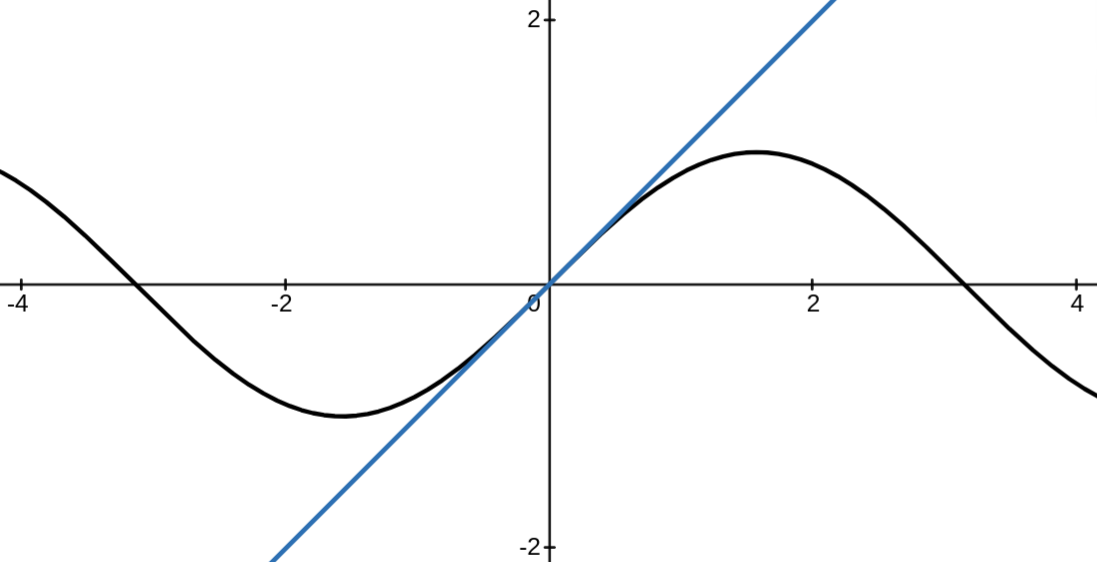
\includegraphics[width=0.7\linewidth]{Pictures/sin1.png}\]
            \[\sin{x}=x+\bar{\bar{o}}{(x)}\]
            \[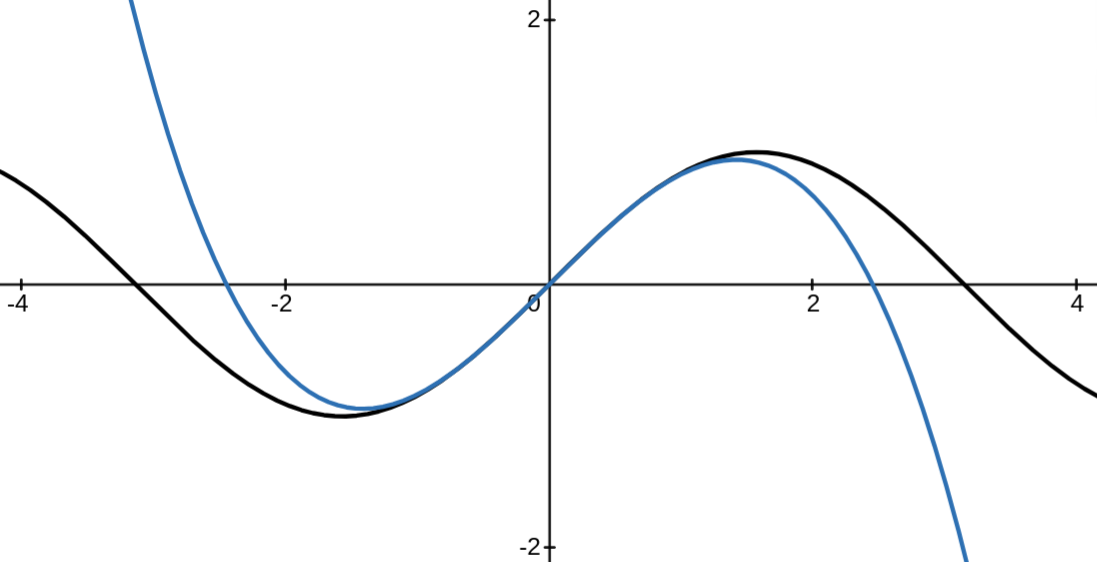
\includegraphics[width=0.7\linewidth]{Pictures/sin2.png}\]
            \[\sin{x}=x-\frac{x^3}{3!}+\bar{\bar{o}}{(x^3)}\]\\
            \[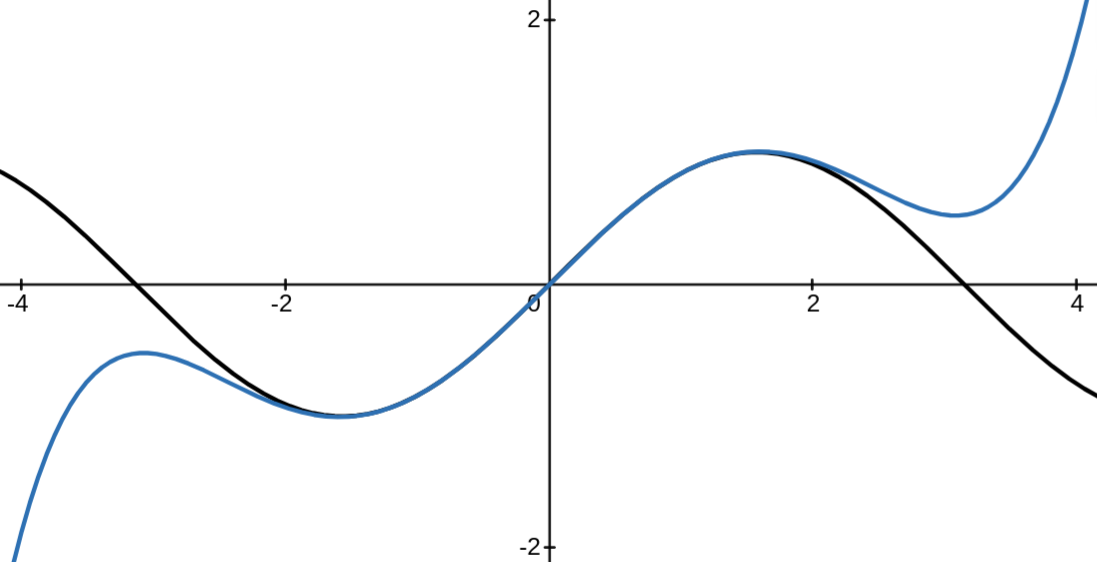
\includegraphics[width=0.7\linewidth]{Pictures/sin3.png}\]
            \[\sin{x}=x-\frac{x^3}{3!}+\frac{x^5}{5!}+\bar{\bar{o}}{(x^5)}\]\\
            \[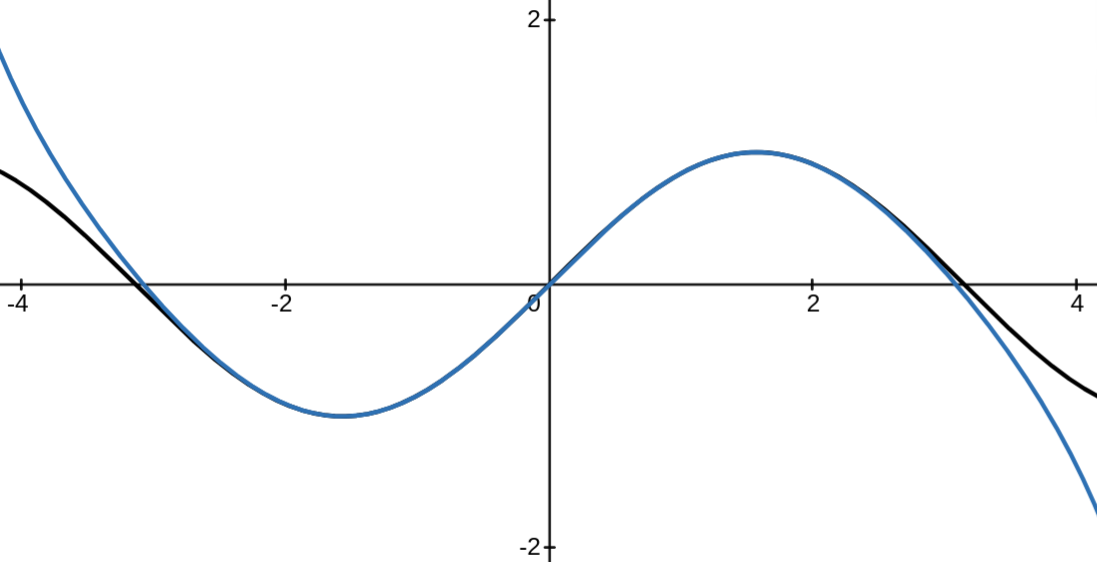
\includegraphics[width=0.7\linewidth]{Pictures/sin4.png}\]
            \[\sin{x}=x-\frac{x^3}{3!}+\frac{x^5}{5!}-\frac{x^7}{7!}+\bar{\bar{o}}{(x^7)}\]
        \end{example}
        \subsection{Экстремум функции}
        \begin{theorem} (Достаточное условие локального экстремума 1)\\
            Пусть $f(x)\in \mathcal{C}(B(x_0)),\ f(x)\in \mathcal{D}(\mathring{B}(x_0))$. \\
            Если при $x<x_0: f'(x)>0$ или при $x>x_0: f'(x)<0$, то $x_0$ - точка максимума.\\
            Если при $x<x_0: f'(x)<0$ или при $x>x_0: f'(x)>0$, то $x_0$ - точка минимума.
        \end{theorem} 
        \begin{proof}
            По формуле Лагранжа: $f(x)-f(x_0)=f'(c)(x-x_0)$
        \end{proof} 
        \begin{theorem} (Достаточное условие локального экстремума 2)\\
            Пусть $\exists\ f^{(n)}(x_0)\ne 0,\ f^{(k)}(x_0)=0,\ k=1, \dots, n-1$.
            \begin{enumerate}
                \item Если $n=2k+1$, то экстремум нет.
                \item Если $n=2k$, то
                \begin{itemize}
                    \item если $f^{(n)}(x_0)>0$, то $x_0$ точка минимум
                    \item если $f^{(n)}(x_0)<0$, то $x_0$ точка максимума.
                \end{itemize}
            \end{enumerate}
        \end{theorem} 
        \begin{proof}
            \[f(x)=f(x_0)+\frac{f^{(n)}(x_0)}{n!}(x-x_0)^n+\bar{\bar{o}}{(x-x_0)^n},\ x\to x_0\]
            \[\Rightarrow f(x)-f(x_0)=(x-x_0)^n(\frac{f^{(n)}(x_0)}{n!}+\bar{\bar{o}}{(1)})\]
            Заметим, что знак $\frac{f^{(n)}(x_0)}{n!}+\bar{\bar{o}}{(1)}$ совпадает со знаком $f^{(n)}(x_0)$ в некоторой проколотой окрестности $x_0$. Значит,
            \begin{enumerate}
                \item Если $n=2k+1$, то $(x-x_0)^n$ меняет знак при переходе $x$ через точку $x_0 \Rightarrow$ при этом переходе $f(x)-f(x_0)$ тоже меняет свой знак $\Rightarrow x_0$ - не экстремум.
                \item Если $n=2k$, то $(x-x_0)^n$ не меняет знак при переходе $x$ через точку $x_0 \Rightarrow$ если $f^{(n)}(x_0)>0$, то $\forall x \in \mathring{B}(x_0): f(x)-f(x_0)>0 \Rightarrow x_0$ - точка минимума. Аналогично при $f^{(n)}(x_0)<0: x_0$ - точка максимума.
            \end{enumerate}
            
        \end{proof} 
        \subsubsection*{Схема поиска глобального экстремума}
        \begin{enumerate}
            \item Ищем точки интервала $(a,b)$, где $f'(x)=0$ или где ее не существует. 
            \item Находим значение во всех этих точках и значения на концах отрезка.
            \item Сравниваем их между собой.
        \end{enumerate}
        \subsection{Выпуклые функции}
        \begin{definition}
            Пусть $f(x)\in \mathcal{C}(I)$. Если $\forall x_1,x_2\in I$ и $\forall x: x_1<x<x_2$:
            \[f(x)\leq \frac{f(x_2)(x-x_1)+f(x_1)(x_2-x)}{x_2-x_1}\]
            то $f(x)$ называется выпуклой вниз. Если выполнено обратное неравенство, то $f(x)$ называется выпуклой вверх. Пример выпуклой вниз функции :
        \end{definition} 
        \begin{center}
            \begin{tikzpicture}[scale=2]
                \draw[->] (-0.5, 0) -- (3.5, 0) node[right] {$x$};
                \draw[->] (0, -0.5) -- (0, 2.5) node[above] {$y$};
                \draw[domain=0.4:3.2,samples=100] plot (\x,{((ln(\x))^2-(0.5*\x)+1.5)});
                \coordinate (x1) at (0.5,0);
                \coordinate (x2) at (3,0);
                \coordinate (y1) at (0.5,1.73);
                \coordinate (y2) at (3,1.2);

                \draw[fill] (x1) circle (1pt) node[below] {$x_1$};
                \draw[fill] (x2) circle (1pt) node[below] {$x_2$};
                \draw[fill] (y1) circle (1pt) node[above right] {$f(x_1)$};
                \draw[fill] (y2) circle (1pt) node[above right] {$f(x_2)$};
                
                \draw[dashed] (x1) -- (y1);
                \draw[dashed] (x2) -- (y2);
                \draw (y1) -- (y2);
            \end{tikzpicture}
        \end{center}
        \begin{theorem} (Достаточное условие выпуклости)\\
            Пусть $f'(x)\in \mathcal{D}(I)$.
            \begin{itemize}
                \item Если $f''(x)>0$, то $f(x)$ выпукла вниз.
                \item Если $f''(x)<0$, то $f(x)$ выпукла вверх.
            \end{itemize}
        \end{theorem} 
        \begin{proof}
            Пусть 
            \[l_1(x)=\frac{f(x_2)(x-x_1)+f(x_1)(x_2-x)}{x_2-x_1}\]
            \begin{multline*}
                f(x)-l_1(x)=\\
                =f(x)\frac{(x-x_1)+(x_2-x)}{x_2-x_1}-\frac{f(x_2)(x-x_1)+f(x_1)(x_2-x)}{x_2-x_1}=\tab[2cm]\\
                \tab[3cm]=\frac{(f(x)-f(x_2))(x-x_1)+(f(x)-f(x_1))(x_2-x)}{x_2-x_1}=\tab[5cm]\\
                \tab[3cm]=\frac{-f'(\xi)(x_2-x)(x-x_1)+f'(\eta)(x-x_1)(x_2-x)}{x_2-x_1}=\\=
                \frac{-f''(\chi)(\xi-\eta)(x-x_1)(x_2-x)}{x_2-x_1}
            \end{multline*}
        \end{proof} 
        \begin{theorem}
            Пусть $f'(x)\in \mathcal{D}(I)$. Если $f''(x)>0\ (f''(x)<0)$, то $\forall x_0\in I$:
            \[f(x)-f(x_0)-f'(x_0)(x-x_0)\geq 0\]
        \end{theorem} 
        \begin{proof}
            Пусть $f(x_0)+f'(x_0)(x-x_0)=l_2(x)$
            \[f(x)-l_2(x)=f'(\xi)(x-x_0)-f'(x_0)(x-x_0)=f''(\eta)(\xi-x_0)(x-x_0)\]
            знаки скобок $(\xi-x_0)$ и $(x-x_0)$ одинаковы, значит $(\xi-x_0)(x-x_0)>0$
        \end{proof} 
        \begin{definition}
            Если $f(x)-l_2(x)$ при проходе через точку $x_0$ меняет знак (разные знаки в левой и правой окрестности), то точка $x_0$ называется точкой перегиба.
        \end{definition}
        \begin{theorem} (Необходимое условие наличия точки перегиба)\\
            Пусть $f''(x)\in \mathcal{C}(B(x_0))$. Если $x_0$ - точка перегиба, то $f''(x_0)=0$.
        \end{theorem}  
        \begin{proof}
            Если $f''(x_0)>0$, то в силу непрерывности $f''(x)>0$ в $B(x_0)$, значит $x_0$ - не точка перегиба. Аналогично для $f''(x_0)<0$.
        \end{proof} 
        \begin{theorem} (Достаточное условие наличия точки перегиба)\\
            Пусть $f''(x)\in \mathcal{C}(I)$. Если $f''(x)$ меняется знак при проходе точки $x_0$, то $x_0$ - точка перегиба.
        \end{theorem} 
        \begin{proof}
            $f(x)-l_2(x)=f''(\eta)(\xi-x_0)(x-x_0)$
        \end{proof} 
        \begin{theorem}
            Пусть $f''(x_0)=0,\ f'''(x_0)\ne 0$. Тогда $x_0$ - точка перегиба.
        \end{theorem} 
        \begin{proof}
            \[f(x)=f(x_0)+f'(x_0)(x-x_0)+\frac{f'''(x_0)}{6}(x-x_0)^3+\bar{\bar{o}}{((x-x_0)^3)}\] 
            Тогда
            \[f(x)-l_2(x)=(x-x_0)^3(\frac{f'''(x_0)}{6}+\bar{\bar{o}}{(1)})\]
        \end{proof} 
        \begin{definition}
            Если при $x\to a-0\ (x\to a+0): f(x)\to \pm \infty$, то прямая $x=a$ называется вертикальной асимптотой.
        \end{definition} 
        \begin{definition}
            Если при $x\to +\infty (x\to -\infty): (f(x)-kx-b)\to 0$, то прямая $y=kx+b$ называется наклонной асимптотой.
        \end{definition} 
        \begin{theorem}
            Прямая $y=kx+b$ является наклонной асимптотой графика функции $f(x) \Leftrightarrow \exists \lim\limits_{x\to +\infty}\frac{f(x)}{x}=k,\ \exists \lim\limits_{x\to +\infty}(f(x)-kx)=b$, аналогично к $-\infty$.
        \end{theorem} 
        \begin{theorem} (Неравенство Йенсена)\\
            Пусть $f(x)$ выпукла вверх в каждой точке $I$. Пусть $\forall i: \alpha_i>0,\ \sum\limits_{i=1}^{n}\alpha_i=1$. Тогда $\forall x_i \subset I$: (Если $f(x)$ выпукла вниз, то выполнено обратное неравенство)
            \[f(\sum\limits_{i=1}^{n}\alpha_i x_i) \geq \sum\limits_{i=1}^{n}\alpha_i f(x_i)\]
        \end{theorem} 
        \begin{proof}
            Индукция по $n$. Если $n=1$ - очев. Для $n=2$ так как $f(x)$ - выпукла вверх: 
            $f(\alpha_1 x_1+\alpha_2 x_2)\geq \alpha_1 f(x_1)+\alpha_2 f(x_2)$
            Пусть верно для $n$. Тогда пользуясь неравенством для $n=1$ и $n=2$ получим:
            \begin{multline*}
                f(\sum\limits_{i=1}^{n+1}\alpha_i x_i)=f(\alpha_{n+1}x_{n+1}+\sum\limits_{i=1}^{n}\alpha_i x_i)=\\
                =f(\alpha_{n+1}x_{n+1}+\sum\limits_{i=1}^{n}\alpha_i \cdot \sum\limits_{i=1}^{n}(\frac{\alpha_i}{\sum\limits_{i=1}^{n}\alpha_i}\cdot x_i))\geq\tab[5cm]\\
                \geq \alpha_{n+1} f(x_{n+1})+\sum\limits_{i=1}^{n}\alpha_i\cdot f(\sum\limits_{i=1}^{n}\frac{\alpha_i}{\sum\limits_{i=1}^{n}\alpha_i} x_i)\geq\\
                \tab[5cm]\geq \alpha_{n+1} f(x_{n+1})+\sum\limits_{i=1}^{n}\alpha_i(\sum\limits_{i=1}^{n}\frac{\alpha_i}{\sum\limits_{i=1}^{n}\alpha_i}\cdot f(x_i))=\\
                =\alpha_{n+1}f(x_{n+1})+\sum\limits_{i=1}^{n}\alpha_i f(x_i)=\sum\limits_{i=1}^{n+1}\alpha_i f(x_i)
            \end{multline*}
        \end{proof} 
        \begin{statement}
            (Неравенство между средним арифметическим и средним геометрическим)
            \[\frac{1}{n}\sum\limits_{k=1}^{n}x_k\geq \sqrt[n]{\prod\limits_{k=1}^{n}x_k}\]
        \end{statement}
        \begin{proof}
            $f(x)=\ln{x},\ f''(x)=-\frac{1}{x^2}<0$ - выпукла вверх. Тогда
            \[\ln({\sum\limits_{k=1}^{n}\frac{x_k}{n}})\geq \frac{1}{n} \sum\limits_{k=1}^{n}\ln{x_k}=\ln({\prod\limits_{i=1}^{n}x_k^{\frac{1}{n}}})\]
            Взяв $\exp$ от обеих частей, получим искомое неравенство.
        \end{proof} 
        \begin{statement}
            (Неравенство Юнга)\\
            $\forall a,b>0,\ \forall p,q>1: \frac{1}{p}+\frac{1}{q}=1$. Тогда 
            \[ab\leq \frac{a^p}{p}+\frac{b^q}{q}\]
        \end{statement}
        \begin{proof}
            Воспользуемся неравенством Йенсена для логарифма:
            \[\ln({\frac{1}{p}\cdot x_1+\frac{1}{q}\cdot x_2})\geq \frac{1}{p}\cdot \ln{x_1}+\frac{1}{q}\cdot \ln{x_2}\]
            $x_1=a^p,\ x_2=b^q$. Тогда
            \[\ln{\frac{a^p}{p}+\frac{b^q}{q}}\geq \ln{a}+\ln{b}=\ln{ab}\]
            Взяв $\exp$ от обеих частей, получим искомое неравенство.
        \end{proof} 